\documentclass[preprint,10pt]{sigplanconf}
\usepackage{amsmath}
\usepackage{amssymb}
\usepackage{graphicx}
\usepackage[british]{babel}
\usepackage{url}
\usepackage{listings}
\usepackage{color}
\usepackage{xspace}

\newcommand{\cL}{{\cal L}}
\newcommand{\TODO}{{\sl TODO \marginpar{\sl TODO}}}
\newcommand{\DTime}{\ensuremath{T}\xspace} % Time dimension
\newcommand{\DeltaDTime}{\ensuremath{\Delta{T}}\xspace}
\newcommand{\DUnitR}{\ensuremath{U_{R}}\xspace} % Unit of measure for resource R
\newcommand{\DeltaDUnitR}{\ensuremath{\Delta U_{R}}\xspace}

\begin{document}
\conferenceinfo{ScalaDays '12}{London, UK.}
\copyrightyear{2012}
\copyrightdata{1-59593-056-6/05/0006}

\titlebanner{DRAFT---Do not distribute}



\title{Aquarium: Billing for the Cloud in the Cloud}

\authorinfo{Georgios Gousios \and Christos KK Loverdos \and Nectarios Koziris}
{GRNET SA}
{\{gousiosg,loverdos,nkoziris\}@grnet.gr}

\maketitle
\begin{abstract}
    This paper describes the architecture for the Aquarium cloud infrastructure
    software. Aquarium is a new software we have built whose main function is to associate cloud resources usage with charging policies.
\end{abstract}

\category{D.2.11}{Software Architectures}{Domain-specific architectures}

\terms
    Algorithms, Performance

\keywords
    Billing, Cloud Computing, Scala, Akka

\section{Introduction}

Public cloud infrastructures have emerged as an alternative to building and
maintaining expensive proprietary data centers. At no upfront investment cost,
companies, especially startups, and individual users rent computing power from
service providers, using the pay-as-you-go charging model and enjoying high
scalability should the requirement arise~\cite{Lourid10}. The use of public cloud
infrastructures is particularly attractive for various forms of research
activities, where budget is usually tight and availability of computing power
can make or break an experiment. An important part of all public clouds is
resource management and customer billing~\cite{Armbr10}. Unfortunately, even
though all proprietary platforms do feature mechanisms for billing customers
for resource usage, there is currently a lack of open solutions.

In this paper we present Aquarium, an open source resource billing software,
designed for handling the production  requirements of {\sc grnet}'s public
Infrastructure as a Service (IaaS) platform. Aquarium utilizes a custom Domain
Specific Language for configuring the supported resources, the pricelists and
the billing algorithms. It receives input from an event queue and presents
billing results through a {\sc rest api}. It has been developed with Scala,
using the Akka library to handle concurrency and actor-based resource
processing. In the following sections, we present the requirements that have driven
Aquarium's design, the software architecture and implementation of important
computational algorithms and a preliminary evaluation of Aquarium's
performance. We also present an account of our experience in introducing Scala
in our company.

\section{Requirements}

Aquarium was designed on a clean sheet to serve a particular purpose,
namely the provision of billing services to an IaaS infrastructure,
and also be extensible to new services. In the following sections,
we briefly present the requirements that shaped Aquarium's design.

\subsection{Application Environment}
Aquarium developed as part of the Okeanos project at GRNet. The
Okeanos project is building a full stack public IaaS system for Greek
universities, and several services on top of it. Several components comprise
the Okeanos infrastructure:

\begin{description}

    \item[Synnefo] is an IaaS management console. Users can create and start
        VMs, monitor their usage, create private internal networks among VMs
        and connect to them over the web. The service backend is based on
        Google's Ganneti for VM host management and hundrends of physical
        VM container nodes.

    \item[Archipelago] is a storage service, based on the Rados
        distributed object store. It is currently under development, and the
        plan is to act as the single point of storage for VM images, shared
        volumes and user files, providing clonable snapshots and distributed
        fault tolerance.
    
    \item[Pithos] is a user oriented file storage service. Currently it its
        second incarnation, it supports content deduplication, sharing of files
        and folders and a multitude of clients.

    \item[Astakos] is an identity consolidation system that also acts as the
        entry point to the entire infrastructure. Users can login using 
        identities from multiple systems, such as the Shibboleth (SAML) 
        federation enabled across all Greek universities or their Twitter 
        accounts.

\end{description}

While all the above systems (and several prospective ones) have different 
user interfaces and provide distinct functionality in the context of
the GRnet IaaS, they all share a common notion of \emph{resources}, access
and manipulation options to which they offer to users. 

\subsection{Sharing}

The Okeanos IaaS will support the Greek higher education, an estimated
population of 100.000 students and researchers. Each member will be granted
access to a collection of resources using her institutional account. To enforce
a limit to the resources that can be acquired from the platform, each user will
have a limited amount of credits, renewable each month, which will be allowed
to spend on any resource available through the infrastructure. Resources can
also be shared; for example files on the Pithos file service or virtual machine
images on the Archipelago storage are potentially subject to concurrent usage from 
multiple users. This means that charges for the use of a single resource
may need to be distributed among several users. Also this may mean that in order
for sharing to work correctly, users may need to transfer credits among them.

\subsection{Resource Limiting}

The Okeanos IaaS will be free service for all users. As such, it is prone to
abuse, either by misappropriating resources or by utilizing resources for
purposes not related to research. A billing system can help with controlling
resource usage if it permits its users to use resources up to a periodically
renewable limit. In order facilitate the development of other infrastructure
system, this limit can be expressed into currency (real or provisional). To
support this scheme, Aquarium will need to update a user's balance almost
immediately after the user has claimed the required resources, and inform other
systems in case the user's credits are exhausted. 

\subsection{Configuration}

Billing systems are by nature open ended. As new services are deployed, new
resources appear, while others might be phased out.  Moreover, changes to
company policies may trigger changes to price lists for those resources, while
ad-hoc requests for large scale computational resources may require special
pricing policies. In order for a billing system to be able to successfully
adapt to changing requirements, it must be able to accommodate such changes
without requiring changes to the application itself. This means that all
information required for Aquarium in order to perform a billing operation,
must be provided to it externally. Moreover, to ensure high-availability,
billing configuration should be updatable while Aquarium is running, or at
least with minimal downtime, without affecting the operation of external
systems.


\subsection{Scaling}

In the context of the Okeanos system, Aquarium provides billing services on a
per user basis for all resources exposed by other systems. As such, it is in
the critical path of user requests that modify resource state; all supported
applications must query Aquarium in order to ensure that the user has enough
credits to create a new resource. This means that for a large number of users
(given previous GRNet systems usage by the Greek research community, we
estimate a concurrency level of 30.000 users), Aquarium must update and
maintain in a queryable form their credit status, 
with soft realtime guarantees. 

Being on the critical path also means that Aquarium must be highly resilient,
too. If Aquarium fails, all supported systems will also fail. Even if Aquarium
fails for a short period of time, it must not loose any billing events, as this
will allow users to use resources without paying for them. Moreover, in case of
failure, Aquarium must not corrupt any billing data under any circumstances,
while it should reach an operating state very fast after a service restart.

\section{Domain Modeling}

\subsection{Basic terminology}
We have already mentioned several entities in our description so far. Let us be a bit more specific on several key terms.

\begin{description}
\item[Credits]
The analog of money. Credits are the `universal money` within Aquarium.

\item[Resource]
A billable/chargeable entity. We generally need credits to use a resource. When a resource is used,  then consume credits. Examples of resources are the \textsf{download bandwidth} and, respectively,  the \textsf{upload bandwidth}, the \textsf{disk space} and the \textsf{VM time} to name a few. Generally speaking, the ``resource'' term specifies the type. A resource may have several properties attached, i.e. it name, unit of measure, a description of how its consumption translates to credit and whether it can have more than one instances.

\item[Resource instance]
A user may have several instances of a resource type. For example, regarding a ``Virtual Machine'' resource, a user may have more then one of them. They are distinguished by their unique resource instance identifier. We call resources that can have more than one instance ``complex'' resources.

\item[Resource event]
An event that is generated by a system, which is responsible for the resource.
The resource event describes a state change for the resource. In particular, a resource event records the time when that state change occurred and the changed value.

\item[Cost policy]
A cost policy refers to a resource and it is the policy used in order to charge credits for resource usage. Cost policies come in three flavors, namely \textsf{continuous}, \textsf{discrete} and \textsf{onoff}.
          
\item[Pricelists] assign a price tag to each resource, within a timeframe.

\item[Charging algorithms] specify the way a resource event can generate consumed credits. 
A charging algorithm can be as simple as a direct multiplication of the 
        chargeable resource quantity with the applicable price. We offer the option, though, to define more complex charging  scenarios, the Aquarium DSL supports a simple imperative language with
        a number of implicit variables (e.g. \texttt{price, volume, date}) 
        that enable administrators to specify, e.g. billing algorithms that
        scale with billable volume. Similarily to price lists, charging algorithms
        have an applicability timeframe attached to them.
        
\item[Credit plans] define a number of credits to give to users and a repetition
        period.

\item[Agreements] assign a name to a charging algorithm, pricelist and creditplan triplets,
        which is then assigned to each user.
        

\item[Resource instance state]
A value which is associated with a resource instance. Usually a floating point number, as in the $10.5$ MB designation regarding a possible ``total current downloading bandwidth''.

\item[User]
An owner of resources and credits. Users are defined externally of Aquarium.

\item[Resource event store]
A datatabase, in the general sense, where resource events are stored.

\item[User bill]
A, usually, periodic statement of how many credits the user has consumed. It may contain detailed analysis that relates consumed credits to resources.
  
\item[Billing period]
A time period at the end of which we issue a user bill.
A billing period is made of a starting date and a duration that is a multiple of a week.
A usual billing period starts on a particular month date (eg. 3rd) and lasts for a month.
Each resource type designates what happens to its accumulated value (if any) at the beginning of the billing period. Usually, at the beginning of the billing period, the accumulating amounts of resources are set accumulating amount. For example, for a monthly billing period, the total uploading bandwidth is reset to zero every month.
   
\item[User state]
The user state is made of the following distinct parts, of which the first two can be integrated to a unifying ``resource'' concept.

\begin{enumerate}
\item User credit state, that is the total credit amount for the user.

\item User resource state, which refers to the state of each resource instance that the user owns.

\item Processing state \TODO
\end{enumerate}

\item[Resource event processing]
The set of algorithmic steps by which a resource event leads to state changes of the user state.

\end{description}

\subsection{Representation of events}
Aquarium is the recipient of several types of events from external systems. More specifically, systems that manage the lifetime and operation of chargeable resources are responsible to send Aquarium events that describe notable resource state changes. As an example, when a user consumes disk space, Pithos, which is the service responsible for user storage, will send a resource event for the \textsf{diskspace} resource and the amount of bytes used.

Another type of events are the user-related events, from the perspective if the Identity Management service. For example, Aquarium needs to know when a user is first created and when the user is activated or suspended. Also, several types of users (e.g. Lab Administrators or Professors in the academic setting where Aquarium is initially targeted for) may be assigned more privileged credit plans that periodically give them more credits.

\begin{figure}
\lstset{language=c, basicstyle=\footnotesize,
stringstyle=\ttfamily, 
flexiblecolumns=true, aboveskip=-0.9em, belowskip=0em, lineskip=0em}

\begin{lstlisting}
abstract class AquariumEvent(
  val id: String,
  val occurredMillis: Long,
  val receivedMillis: Long)
  
case class ResourceEvent(
    override val id: String,
    override val occurredMillis: Long, 
    override val receivedMillis: Long, 
    userId: String,
    clientId: String,               
    resource: String,
    value: Double,
    details: Map[String, String])
  extends AquariumEvent(id, occurredMillis, receivedMillis)
\end{lstlisting}
\caption{Representation of events in Scala.}
\label{fig:aqevent}
\end{figure}

The actual format of the event is presented in Figure~\ref{fig:resevt}.

\begin{figure}
\lstset{language=C, basicstyle=\footnotesize,
stringstyle=\ttfamily, 
flexiblecolumns=true, aboveskip=-0.9em, belowskip=0em, lineskip=0em}

\begin{lstlisting}
{
  "id":"4b3288b57e5c1b08a67147c495e54a68655fdab8",
  "occuredMillis":1314829876295,
  "receivedMillis":1314829876300,
  "userId": "31",
  "cliendId": "snf-astakos-1",
  "resource": "vmtime",
  "value": 1,
  "details": {
    "vmid": "3300",
    "action": "on"
  }
}
\end{lstlisting}
\caption{A JSON-formatted \texttt{ResourceEvent}} 
\label{fig:resevt}
\end{figure}

For the exchange of events we adopt the ubiquitous JSON format. This is chosen for the ease of manipulation from both Scala, used in Aquarium, and Python, used for the rest of the communicating systems. Our base entity, \texttt{AquariumEvent} and the \texttt{ResourceEvent} corresponding to a resource event, as described previously, are shown in Figure~\ref{fig:aqevent}, while Figure~\ref{fig:resevt} presents a JSON-formatted \texttt{ResourceEvent} value. The given attributes are:

\begin{description}
\item[id] is the event \textsf{ID} at the client side, that is the sender of the event. Aquarium requires that \textsf{IDs}

\item[occurredMillis] gives us the time of when the even occurred, using the Unix time convention.

\item[receivedMillis] gives us the time of when the event was received in the Aquarium processing pipeline, also using the Unix time convention.

\item[userId] is the unique identifier of the user this event relates to. Use identifiers are managed by the Identity Management system, Astakos.

\item[clientId] is a unique, across all systems, identifier for the external system generating the event.

\item[resource] is the resource name.

\item[value] is the resource's changed value.

\item[details] is a resource-specific collection of  attributes and their values.
\end{description}

Of particular interest is the \textsf{details} map. Several resource types can use this map in order to pass resource-specific attributes to Aquarium, which in turn can be hooked into the charging algorithm. We motivate this extension mechanism with an example for the \textsf{vmtime} resource type, which simply represents usage of virtual machines. A respective resource event needs to specify:
\begin{itemize}
\item Which particular resource instance (which virtual machine) it refers to.
\item The relevant state change for the resource instance. In this case, a virtual machine can be started (\textsf{on} state) or stopped (\textsf{off} state).
\end{itemize}

In our example of Figure~\ref{fig:resevt}, we use the \textsf{vmId} and \textsf{action} extensions to specify that the virtual machine instance with identifier \textsf{3300} was started, that is it transitioned to \textsf{on} state. We should generally note that each resource type is free to choose the domain-specific description for the instance \textsf{ID}. 

Finally, for the timing of events we assume all systems that send event to Aquarium have synchronized clocks. We actually \textit{require} this, so that Aquarium is not concerned with time book keeping.


\subsection{The configuration DSL}
\label{sec:dsl}
We addressed the configuration requirements of Aquarium by creating a new
domain specific language ({\sc dsl}), based on the YAML format.  The DSL
enables administrators to specify chargeable resources, charging policies and
price lists and combine them arbitrarily into agreements applicable to specific
users, user groups or the whole system. 
The DSL supports inheritance for policies, price lists and agreements and composition in the case of agreements.
It also facilitates the
definition of generic, repeatable debiting rules, which are then used by the
system to refill the user's account with credits on a periodic base.

From the previously specified term, the following five are used in the DSL:

\begin{enumerate}
\item Resources
\item Charging algorithms
\item Price lists
\item Credit plans
\item Agreements
\end{enumerate}


\begin{figure}
\lstset{language=c, basicstyle=\footnotesize,
stringstyle=\ttfamily, 
flexiblecolumns=true, aboveskip=-0.9em, belowskip=0em, lineskip=0em}

\begin{lstlisting}
resources:
  - resource:
    name: bandwidthup
    unit: MB/hr
    complex: false
    costpolicy: continuous
pricelists:
  - pricelist: 
    name: default
    bandwidthup: 0.01
    effective:
      from: 0
  - pricelist: 
    name: everyTue2
    overrides: default
    bandwidthup: 0.1
    effective:
      repeat:
      - start: "00 02 * * Tue"
        end:   "00 02 * * Wed"
      from: 1326041177        //Sun, 8 Jan 2012 18:46:27 EET
algorithms:
  - algorithm:
    name: default
    bandwidthup: $price times $volume
    effective:
      from: 0
agreements:
  - agreement:
    name: scaledbandwidth
    pricelist: everyTue2
    algorithm:
      bandwidthup: |
        if $volume gt 15 then
          $volume times $price
        elsif $volume gt 15 and volume lt 30 then
          $volume times $price times 1.2
        else
          $volume times price times 1.4
        end
\end{lstlisting}

\caption{A simple billing policy definition.} 
\label{fig:dsl}
\end{figure}

In Figure~\ref{fig:dsl}, we present the definition of a simple (albeit valid) 
policy. The policy parsing is done top down, so the order of definition 
is important. The definition starts with a resource, whose name is then
re-used in order to attach a pricelist and a price calculation algorith to it.
In the case of pricelists, we present an example of \emph{temporal overloading};
the \texttt{everyTue2} pricelist overrides the default one, but only for 
all repeating time frames between every Tuesday at 02:00 and Wednesday at
02:00, starting from the timestamp indicated at the \texttt{from} field. Another
example of overloading is presented at the definition of the agreement, which
overloads the default algorithm definition using the imperative part of the
Aquarium {\sc dsl} to provide a scaling charge algorithm.

\section{Architecture}
\paragraph{Architectural decisions} As most in similar systems, Aquarium's architectural design is driven by two 
requirements: scaling and fault tolerance. As described in the requirements
section above, the concurrency and responsiveness requirements are steep;

Driven by our former experience with 3 tier systems, we designed the first
Aquarium prototype around a traditional relational database backend, with an
object relational mapping ({\sc orm}) based middle layer that run the business
processes (billing, message processing etc) and a fully-fledged {\sc rest}
frontend. While the simplicity of {\sc orm} systems provided a great start,
it quickly became obvious that such a design was too rigid for an open 
ended system. Complications arised from the fact that it was too difficult
to describe versioned tree-based structures, such as the configuration {\sc dsl} 
(see Section~\ref{sec:dsl}) and to make sure that resource events were
described in an abstract way that would include all future system expansions.
Moreover, the single query that places Aquarium in the system's critical 
path (number of remaining credits) must be answered within a few (less than
10) milliseconds for a large number of concurrent requests, which means that
it must be somehow cached and automatically updated when new chargable 
resources are invoked by the user.

For the reasons outlined above, we chose to base Aquarium on event sourcing. 
Event sourcing assumes that all changes to application
state are stored as a sequence of events, in an immutable log. With such a log
at hand, a system can easily rebuild the current state by replaying the events
in order. The event sourcing design pattern has some very interesting
properties, which made it particularity suitable for basing Aquarium's
architecture on it:

\begin{itemize}

    \item Multiple models can be used in order to process the events, 
        concurrently. This means that Aquarium can provide a limited
        data view to its {\sc rest api} and a more detailed one to a
        helpdesk frontend.

    \item It is possible to perform queries on past system states by stopping
        the event replay at a certain point of interest. This would prove very
        possible for a future debugging interface.

    \item In a carefully implemented event sourcing system, application crashes 
        are not destructive, as long as event replay is fast enough and no
        state is inserted to the application without being recorded to the event
        log first.

    \item After event log replay, new events only cause updates in the system's
        in-memory state, which can be done very fast.

\end{itemize}

\begin{figure}
    \begin{center}
    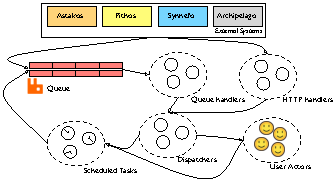
\includegraphics[scale=1.5]{arch.pdf}
    \end{center}
\caption{Functional components in Aquarium's architecture} 
\label{fig:arch}
\end{figure}

With event sourcing as the basis for Aquarium, we then proceeded to design the
system's runtime data model. What we wanted to model was the current state of
resource usage for each user, along with the user's wallet. One possibility we
wanted to explore on that front was copy on write updates; even for trivial
updates, the system would have to copy the affected data graphs to new
versions, instead of modifying the system in place. For that, we briefly
explored the use of software transactional memory, but found it restrictive for
our pursposes. What we chose instead was to contain each user's runtime state
in an actor. Using this design, shared state was eliminated; the use of the
actor model guarantee, that only one thread can execute within the context of
an actor renders the protection (with copy on write or other mechanism) of the
actor's state superflous. The actor model also fitted the event sourcing basis
very well, since each message in the log could pass through various processing
stages and reach the appropriate actor immutably.

\paragraph{Components} An overview of the Aquarium architecture is presented in
Figure~\ref{fig:arch}.  The system is modeled as a collection of logically and
functionally isolated components, which communicate by message passing. Withing
each component, a number of actors take care of concurrently processing
incoming messages through a load balancer component which is the gateway to
requests targeted to the component. Each component is also monitored by its own
supervisor; should an actor fail, the supervisor will automatically restart it.
The architecture allows certain application paths to fail individually while
the system is still responsive, while also enabling future distribution of
multiple components on clusters of machines.

The system receives input mainly from two sources: a queue for resource and
user events and a {\sc rest api} for billing state queries. The queue component
reads messages from a configurable number of queues and persists them in the
application's immutable log store. Both input components then forward incoming
messages to a network of dispatcher handlers which do not do any processing by
themselves, but know where the user actors lay. As described earlier, actual
processing of billing events is done within the user actors. Finally, a
separate network of actors take care of scheduling periodic tasks, such as
refiling of user credits; it does so by issuing events in the appropriate
queue.

\paragraph{Implementation}

Aquarium is being developed as a standalone service, based on the Akka library
for handling actor related functionality. Akka has all basic components for
implementing the architecture as described, which allowed us to focus on
implementing the business logic, leaving the details of actor registries,
dispatchers and message passing to Akka's runtime. Akka also provided
actor-based components for communicating with the message queue and, through a
third party component (Spray)\footnote{\url{http://github.com/spray}} for
handling {\sc rest} requests.  We chose the {\sc amqp} protocol and its
Rabbit{\sc mq} implementation for implementing the request queue, specifically
because recent versions include support for active/active cluster
configurations. The persistence layer is currently implemented by Mongo{\sc
db}, for its replication and sharding support.  However, this is not a hard
requirement, as Aquarium features an abstraction layer for all database queries
(currently 10 methods), which can then be implemented by any persistence
system, relational or not.


\section{Computational aspects}

\subsection{Charging basics}
The previously mentioned DSL gives us a declarative way of describing the charging algorithms and the other related concepts. The computational engine of Aquarium then transforms these declarations to computing steps for the charging process.

Charging, based on a resource event, is inherently multidimensional. Time (\DTime) is always one dimension to consider: there are resources whose charging is based on the passing of time. Also, rather obviously, the unit of measure (\DUnitR) for a resource ($R$) is yet another dimension to take into account. These dimensions usually enter the formulas of the charging algorithms, although it is not necessary that all of them do. But there is one more aspect to consider, which clearly adds up to the multidimensionality of the problem. More specifically, \DUnitR can be taken into account either as whole value or as a difference \DeltaDUnitR. An avid reader may be already wondering about time. Shouldn't it be treated in the same footing, at least for reasons of conceptual uniformity? Shouldn't we treat both \DTime and \DeltaDTime? In reality, we \textit{always} work with time differences. Usually, \DeltaDTime means the time difference between two resource events for the same resource instance. In such a setting, \DTime would mean the time difference from some well-known and predefined point in time. This is generally a possibility, for example by considering the beginning of a billing period as the beginning of time as far as a particular charging calculation is concerned. So all combinations of either full values or differences can be considered, as given in Table~\ref{tab:dt}.

\begin{table}[htdp]
\label{tab:dt}
\begin{center}
\begin{tabular}{|c|c|c|}
\hline
&Time & Resource unit of measure \\
\hline
Absolute value & \DTime & \DUnitR \\
Difference & \DeltaDTime  & \DeltaDUnitR \\
\hline
\end{tabular}
\end{center}
\label{default}
\caption{Considering time and resource unit of measure as absolute values or differences
}
\end{table}%


Now, we can take this reasoning a bit further, by 

Per resource, the charging operation is affected by the cost policy and complexity
parameters. Specifically, the 3 available cost policies affect the calculation 
of the amount of resource usage to be charged as follows:

\begin{itemize}
    \item resources employing the \textsf{continuous} cost policy are charged for
        the actual resource usage through time. When a resource event arrives,
        the previous resource state between the previous charge operation and the
        current event event timestamp is charged and the resource state is then
        updated. More formally, for continuous resources, if $f(t)$ represents
        the function of resource usage through time and $p(t)$ is the function
        representing the pricelist at time $t$, 
        then the total cost up to a 
        $c(t) = \sum_{i=0}^{t} {p(t) \times \int_0^{t}{f(t)dt}}$. Most resources
        in Aquarium are continuous, for example bandwidth and disk space.

    \item resources employing the \textsf{onoff} cost policy can be in two states:
        either switched on and actively used or switched off. Therefore, the unit
        of resource usage is time and not the actual resource usage, while the
        period of charging is calculated only when the resource is switched on.
        Virtual machines are examples of resources with the \textsf{onoff} cost
        policy.

    \item resources using the \textsf{distinct} cost policy are charged
        upon usage, without time playing a role in the charge. Such resources
        are useful for one off charges, such as the allocation of
        virtual machine or the migration of a virtual machine to a less busy
        host.

\end{itemize}


\subsection{State management}
Commonly to most similar systems, billing in Aquarium is the application of the
provisions of a user's contract to an incoming billing event in order to
produce an entry for the user's wallet. However, in stark contrast to most
other systems, which rely on database transactions in order to securely modify
the user's balance, Aquarium performs account updates asynchronously and
concurrently for all users.

Billing events are obtained through a connection to a message queue. Upon
arrival, a billing event is stored in an immutable log, and then forwarded to
the user actor's mailbox; the calculation of the actual billing entries to be
stored in the user's wallet is done within the context of the user actor,
serially for each incoming events. This permits the actor to have mutable state
internally (as described in Section~\ref{sec:ustate}), without risking the
calculation correctness. The calculation process involves steps such as
validating the resource event, resolving the current state of resource affected
by the incoming resource event, deciding the value applicable pricelist and
algorithm, generating entries for the user's wallet and updating the current
resource state for the user. A significant source of complexity in the process
is the support for temporal overriding for pricelists and algorithms: within
the timeframe between resource updates, several policies or algorithms may be
active. The billing algorithm must therefore split the billing period to pieces
according the applicability of each policy/algorithm and make sure that at 
least a baseline policy is in effect in order to perform the calculation.
Consequently, a resource event might lead to several entries to the user's wallet.

\subsection{User State}
\label{sec:ustate}

\section{Performance}

To evaluate the performance of Aquarium, we formulated an experiment that
evaluated two important properties: the time required to perform the charging
operation for a resource event and the overall time required to process a
resource event, end to end. To conduct the experiment, Aquarium was configured,
using the policy {\sc dsl} to handle billing events for 5 types of resources,
using 3 overloaded pricelists, 2 overloaded algorithms, all of which were
combined to 5 different agreements. Aquarium's data store was pre-filled in
with 1.000.000 resource events, evenly distributed among 1.000 users. To drive
the benchmark, we used a synthetic load generator that produced random
billing events, at a configurable rate per minute. 

To run the benchmark, we deployed Aquarium on a virtualized 4 core 2{\sc gh}z
class {\sc cpu} and 4{\sc gb} {\sc ram} Debian Linux server, on the Okeanos
cloud infrastructure. The virtual machine running Aquarium was configured with
a 4{\sc gb} maximum heap size. We selected Rabbit{\sc mq} and Mongo{\sc db} as
the queue and database server respectively, both of which where run in another
4-core, 4{\sc gb ram} virtual machine. Both systems were run using current
versions at the time of benchmarking (2.7.1 for Rabbit{\sc mq} and 2.6 for
Mongo{\sc db}). The two virtual machines did not share a physical host and
communicated over Okeanos's switched network fabric at an effective rate of 800
Mbits/sec, as reported by the \texttt{iperf} utility.  We paid particular
attention to have Mongo{\sc db} load the full working data set in memory, by
repeatedly querying all stored records. No further optimization was performed
on either back-end system.

\begin{figure}[t]
    \begin{center}
        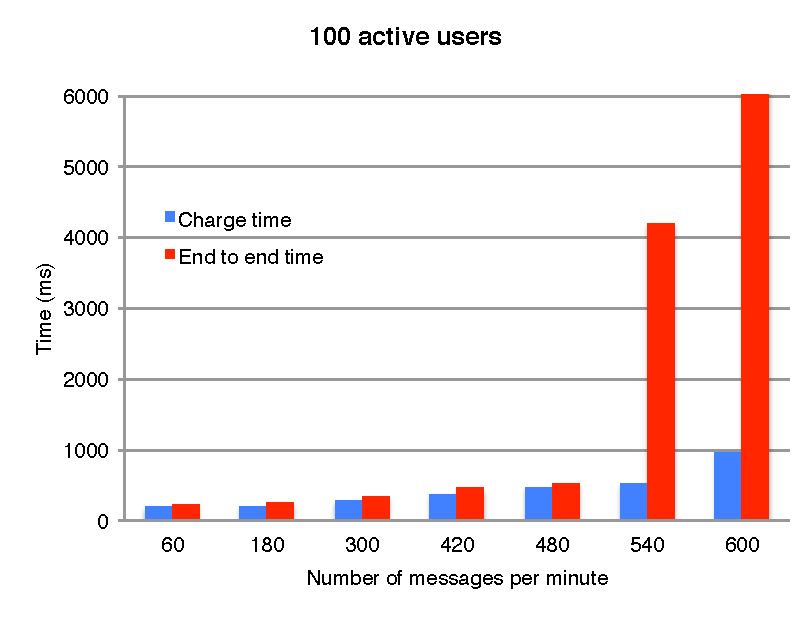
\includegraphics[scale=0.63]{perf.pdf}
    \end{center}

    \caption{Average time for peforming a billing operation and end for end to
    end message processing for 100 active users and a varying number of
    messages per minute.}
    
    \label{fig:perf}
\end{figure}

All measurements were done using the first working version of the Aquarium
deployment, so no real optimisation effort has taken place. This shows in the
current performance measurements, as Aquarium was not able to handle more that
about 500 billing operations per second. One factor that contributed to this
result was the way resource state recalculations was done; in the current
version, the system needs to re-read parts of the event and billing state from
the database every time a new resource event appears. This contributes to more
than 50\% of the time required to produce a charging event, and can be
completely eliminated when proper billing snapshots are implemented. In other
measurements, we also observed that the rate of garbage creation was extremely
high, more that 250 {\sc mb/sec}. Upon further investigation, we attributed it
to the way policy timeslot applicability is calculated. Despite the high
allocation rate, the {\sc jvm}'s garbage collector never went through a
full collection cycle; when we forced one after the benchmark run was over, 
we observed that the actual heap memory usage was only 80{\sc mb}, which
amounts to less than 1 {\sc mb} user.

Even so, by extrapolating on the results and hardware configuration, an average
12-core box could handle more 1.500 messages per minute from about 300 active
users, at 5 events per minute. Given that activity from users is expected to
arrive in bursts, a more realistic expectation might be to receive 1 message
per user per 5 minutes on average; in that case, and provided that the resource
query cost is negligible as it is being served from an in memory cache, the
system could handle around 4.500 concurrent users. While such back of the
envelop calculations do not account for traffic spikes, they do provide an
rough estimation of the optimisation effort that must be put in place. 


\section{Lessons Learned}

One of the topics of debate while designing Aquarium was the choice of
programming platform to use. With all user facing systems in the Okeanos cloud
being developed in Python and the initial Aquarium designers being beginner
Scala users (but experts in Java), the choice certainly involved risk that
management was initially reluctant to take. However, by breaking down the
requirements and considering the various safeguards that the software would
need to employ in order to satisfy them, it became clear that a
typesafe language was a hard requirement. Of the platforms examined, the {\sc
jvm} had the richest collection of ready made components; the Akka library was
particularly enticing for the scalability and distribution possibilities it
offered.

The choice of Scala at the moment it had been made was a high risk/high gain
bet for GRNet. However, the development team's experience has been generally
positive. Scala as a language was an enabling factor; case classes permitted
the expression of data models, including the configuration {\sc dsl}, that
could be easily be serialized or read back from wire formats while also
promoting immutability through the use of the \texttt{copy()} constructor. The
pervasive use of immutability allowed us to write strict, yet simple and
concise unit tests, as the number of cases to be examined was generally low.
The \textsf{Maybe}\footnote{\textsf{Maybe} works like \textsf{Option}, but it
has an extra possible state (\textsf{Failed}), which allows exceptions to be
encapsulated in the return type of a function, and then retrieved and accounted
for in a pattern matching operation with no side effects. More at
\url{https://github.com/loverdos/Maybe}} monad, enabled side-effect free
development of data processing functions, even in cases where exceptions were
the only way to go. Java interoperability was excellent, while thin Scala
wrappers around existing Java libraries enabled higher productivity and use of
Scala idioms in conjunction with Java code.

The Akka library, which is the backbone of our system, is a prime example of 
the simplicity that can be achieved by using carefully designed high-level
components. Akka's custom supervision hierarchies allowed us to partition the
system in self-healing sub-components, each of which can fail independently
of the other. For example, if the queue reader component fails due to a queue
failure, Aquarium will still be accessible and responsive for the {\sc rest}
interface. Also, Akka allowed us to easily saturate the processing components
of any system we tested Aquarium on, simply by tuning the number of threads (in
{\sc i/o} bound parts) and actors (in {\sc cpu} bound parts) per dispatcher. 

Despite the above, the experience was not as smooth as initially expected. The
most prominent problem we encountered was that of lacking documentation. The
Akka library documentation, extensive as is, only scratches the surface.
Several other libraries we use, for example Spray for {\sc rest} handling, have
non-existent documentation. The Java platform, and .Net that followed, has
shown that thorough and precise documentation are key to adoption, and we
expected a similar quality level. Related is the problem of shared community
wisdom; as most developers know, a search for any programming problem will
reveal several straightforward Java or scripting language sources. The
situation with Scala is usually the opposite; the expressive power of the
language makes it the current language of choice for treating esoteric
functional programming concepts, while simple topics are often neglected. Scala
has several libraries of algebraic datatypes but no {\sc yaml} parser. As Scala
gains mainstream adoption, we hope that such problems will fade.

From a software engineering point of view, the current state of the project was
reached using about 6 person months of effort, 2 of which were devoted to
requirements elicitation, prototype building and familiarizing with the
language. The source code currently consists of 5.000 lines of executable
statements (including about 1.000 lines of tests), divided in about 10
packages. The system is built using both {\sc sbt} and Maven. 


\section{Related Work}

While IaaS offerings are cheap, they are not free. Service provisioning
incurs costs that service providers must charge to users. Yousef et
al.~\cite{Youse08} described the three pricing models that are used by cloud
service providers for billing used resources, namely tiered pricing, per-unit
pricing and subscription-based pricing. Aquarium's cost policies that are
assigned to resources map exactly to Yousef's pricing models. In fact,
most offerings by public IaaS providers~\cite{Azure12, Amaz12} offer
services charged according to Yousef models.

A lot of research work on resource accounting and billing has been carried out
in the context cloud federation~\cite{Rochw09, Elmro09} and (earlier) grid
federation projects. The Distributed Grid Accounting System ({\sc
dgas})~\cite{Piro06} was among the first to enable resource accounting at the
computing and storage layers and then aggregation of the resources in a
centralized location. The {\sc dgas} system was then adopted by the {\sc egee}
project that provided federation of grid computing resources among European
institutions. The Reservoir project investigated the use of service level
agreements~\cite{Elmro09} for resource provisioning in federated cloud
scenarios. Resource monitoring and billing are identified as key
functionalities for such services, however, no actual implementation was
produced.

On the cloud computing front, vendors such as VMWare, Microsoft and {\sc ibm}
provide full stack solutions, which also include resource accounting. Usually,
such systems are connected with existing enterprise resource planning systems
\"Ubersmith has developed an engine dedicated to resource accounting; much like
Aquarium, it is tracks resource usage and applies accounting policies to it.
On the open source front, neither the Cloustack nor the Openstack projects,
have yet incorporated billing into their services. To the best of our
knowledge, Aquarium is the first freely available system to offer configurable
accounting services for IaaS deployments.

\section{Conclusions and Future Work}

In this paper, we presented Aquarium, a generic billing system, currently tuned
for cloud resource billing. We presented the requirements that underpinned its
design, outlined the architectural decisions made and analysed its
implementation and performance.
Scala has been an enabling factor for the
implementation of Aquarium, both at the system prototyping phase and during
actual development.  

Aquarium is still under development; a first stable version will be available
in mid-2012, with an service deployment being planned for February 2012. 
The majority of features described in this paper have already been developed.
Future work includes optimization and fine tuning, along with user interfaces
for retrieving account state by end users.
It is available under the {\sc bsd} license at 
\url{https://code.grnet.gr/projects/aquarium}.

\bibliographystyle{abbrvnat}
\bibliography{aquarium}

\end{document}
